%%%%%%%%%%%%%%%%%%%%%%%%%%%%%%%%%%%%%%%%%
% The Legrand Orange Book
% LaTeX Template
% Version 2.1.1 (14/2/16)
%
% This template has been downloaded from:
% http://www.LaTeXTemplates.com
%
% Original author:
% Mathias Legrand (legrand.mathias@gmail.com) with modifications by:
% Vel (vel@latextemplates.com)
%
% License:
% CC BY-NC-SA 3.0 (http://creativecommons.org/licenses/by-nc-sa/3.0/)
%
% Compiling this template:
% This template uses biber for its bibliography and makeindex for its index.
% When you first open the template, compile it from the command line with the 
% commands below to make sure your LaTeX distribution is configured correctly:
%
% 1) pdflatex main
% 2) makeindex main.idx -s StyleInd.ist
% 3) biber main
% 4) pdflatex main x 2
%
% After this, when you wish to update the bibliography/index use the appropriate
% command above and make sure to compile with pdflatex several times 
% afterwards to propagate your changes to the document.
%
% This template also uses a number of packages which may need to be
% updated to the newest versions for the template to compile. It is strongly
% recommended you update your LaTeX distribution if you have any
% compilation errors.
%
% Important note:
% Chapter heading images should have a 2:1 width:height ratio,
% e.g. 920px width and 460px height.
%
%%%%%%%%%%%%%%%%%%%%%%%%%%%%%%%%%%%%%%%%%

%----------------------------------------------------------------------------------------
%	PACKAGES AND OTHER DOCUMENT CONFIGURATIONS
%----------------------------------------------------------------------------------------

\documentclass[11pt,fleqn]{book} % Default font size and left-justified equations

\usepackage{ifthen} 
\newboolean{VersionProf}
\setboolean{VersionProf}{false}

\usepackage{wasysym}
\usepackage{esint} % various fancy integral symbols
\usepackage{tikz}
\usepackage{tikz-3dplot}
\usepackage{pgfplots}
\pgfplotsset{compat=1.17}
\usetikzlibrary{patterns}
\usepackage{tkz-euclide} 
\usepackage{mathtools}
\usepackage{xurl}
\usepackage[version=4,arrows=pgf-filled,
textfontname=sffamily,
mathfontname=mathsf]{mhchem}
\usepackage{gensymb}
\usepackage{tabularray}
\usepackage{csquotes}

\usepackage[french]{babel}
\usepackage{dingbat}

\usepackage{environ}
\usepackage{wrapfig}

\NewEnviron{solution}{%
    \ifthenelse{\boolean{VersionProf}}{\begin{solutionA}
        \BODY%*
        \end{solutionA}
    }{%
        \relax%
    }%
}%

\usetikzlibrary {arrows.meta} 

\newcommand{\degC}{{\degree}C}
\newcommand{\dd}{\mathrm{d}}
\newcommand{\div}{\mathrm{div}}
\newcommand{\rot}{\vv{\mathrm{div}}}
\newcommand{\grad}{\vv{\mathrm{grad}}}

\tikzset{
    support/.style={
        pattern=north east lines,
        draw=none,
        minimum width=0.3,
        minimum height=0.6
    }
    ,>=latex
}

\usepackage[d]{esvect}

%SPECIFIC TO THIS CHAPTER
\usepackage{physics}
\usepackage{ifthen}
\usepackage[outline]{contour} % glow around text
\usetikzlibrary{calc} % for pic
\usetikzlibrary{angles,quotes} % for pic
\usetikzlibrary{patterns}
\tikzset{>=latex} % for LaTeX arrow head
\contourlength{1.2pt}

\colorlet{myred}{red!65!black}
\definecolor{myred}{RGB}{127,0,255}
\tikzstyle{ground}=[preaction={fill,top color=black!10,bottom color=black!5,shading angle=20},
                    fill,pattern=north east lines,draw=none,minimum width=0.3,minimum height=0.6]
\tikzstyle{mass}=[line width=0.6,myred,fill=myred!40,rounded corners=1,
                  top color=myred!40,bottom color=myred!20,shading angle=20]
\tikzstyle{rope}=[myred!30,line width=1.2,line cap=round] %very thick

% FORCES SWITCH
\tikzstyle{force}=[->,myred,ultra thick,line cap=round]
\tikzstyle{Fproj}=[force,myred!60]
\newboolean{showforces}
\setboolean{showforces}{true}
%----------------------------------------------------------------------------------------

\input{structure} % Insert the commands.tex file which contains the majority of the structure behind the template

\begin{document}

%----------------------------------------------------------------------------------------
%	TABLE OF CONTENTS
%----------------------------------------------------------------------------------------

%\usechapterimagefalse % If you don't want to include a chapter image, use this to toggle images off - it can be enabled later with \usechapterimagetrue

\chapterimage{filmB.jpg} % Table of contents heading image

%\pagestyle{empty} % No headers

%\tableofcontents % Print the table of contents itself

%\cleardoublepage % Forces the first chapter to start on an odd page so it's on the right

%\pagestyle{fancy} % Print headers again



%\part{\'{E}lectromagnétisme}

\setcounter{chapter}{8}

\chapter{Interférences par division d'amplitude}

\section{Lame d'air, irisations et teintes de Newton}

\subsection{Introduction}

L'un des phénomènes les plus courants permettant d'observer des interférences lumineuses correspond à la présence d'irisations. Ces irisations peuvent être observées sur un film de savon (comme sur l'image de haut de page, où un écoulement crée des structures turbulentes), mais également à la surface d'une goutte d'huile qui se répand sur une flaque d'eau, ou encore sur les ailes des papillons.

Ces différents systèmes ont tous une même propriété : ils correspondent à des interférences par division d'amplitude.
\begin{definition}[Interférences par division d'amplitude]
On parle d'interférences par divions d'amplitude lorsqu'en un point $M$ d'observation, les deux rayons qui interfèrent sont issus d'un même rayon lumineux initial.
\end{definition}

C'est ce que l'on observe ici : les irisations correspondent à une figure d'interférences qui se produit entre un rayon lumineux réfléchi au niveau d'un premier dioptre, et un rayon réfléchi au niveau d'un second dioptre, comme indiqué sur la figure. Il y a alors une différence de marche entre les deux rayons lumineux, qui produit des interférences. Cette configuration correspond à ce que l'on appelle la lame d'air, et on va étudier ce dispositif plus en détail.


\begin{figure}[htbp]
	\centering 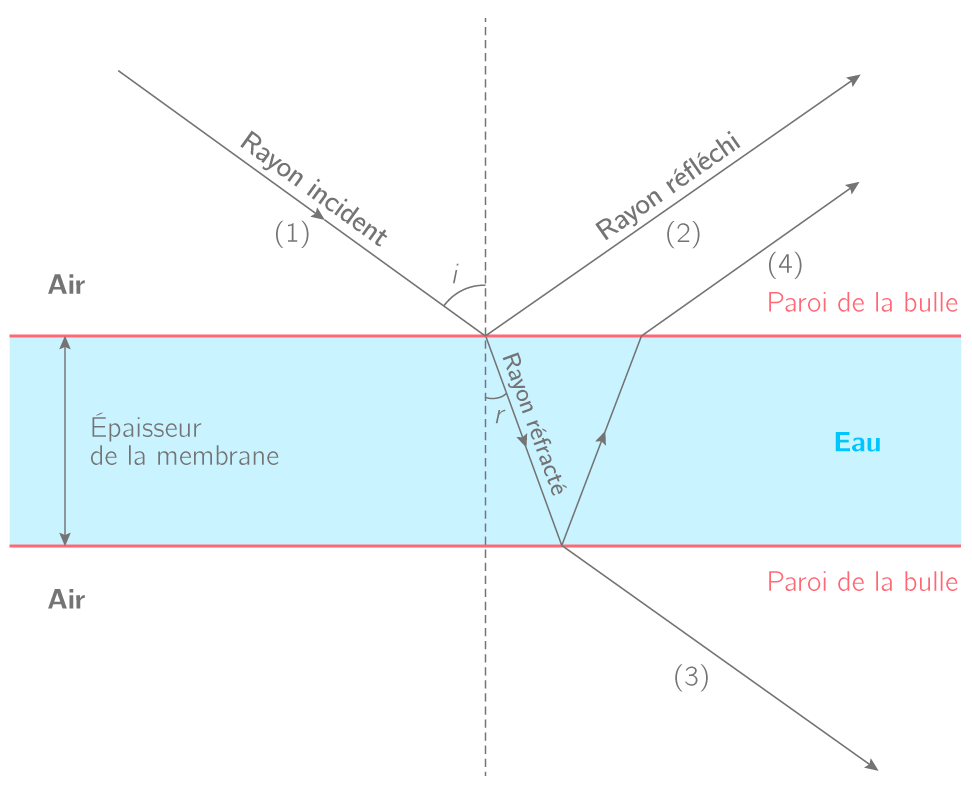
\includegraphics[width=0.8\linewidth]{lame_air_schema.png}
	\caption{Schéma d'un film de savon. Les rayons optiques subissent des trajectoires similaires dans le cas d'un film d'huile, ou d'air.}
\end{figure}

\subsection{Interférences pour une lame d'air}

\subsubsection{Lumière monochromatique}

On peut regarder de plus près la mince couche qui est la cause des interférences. On supposera qu'il s'agit d'un film de savon, dont l'indice optique peut être assimilé à celui de l'eau. On cherche à calculer la différence de marche, à l'infini, entre les deux rayons qui interfèrent.

\begin{capex}
	Déterminer la différence de marche entre les deux rayons émergents (3), en notant $n$ l'indice de la lame, $e$ son épaisseur, et $i$ l'angle d'incidence. On supposera la lumière monochromatique et on notera $\lambda$ sa longueur d'onde. En déduire l'allure des figures d'interférences observées en incidence quasi-normale (loin des surfaces concernées).
\end{capex}

Lorsque $e=0$, les deux rayons ont parcouru (de manière évidente) le même chemin optique. On dit qu'il y a \textit{contact optique}, et on peut alors observer une frange brillante. Pour caractériser les autres franges, on définit l'ordre d'interférence :
\begin{definition}[Ordre d'interférence]
L'ordre d'interférence d'une frange, noté $p$, correspond au nombre de franges entre le contact optique et la frange concernée. Il est donné par la formule suivante :
	\begin{equation}
		p = \frac{\delta(M)}{\lambda}
	\end{equation}
\end{definition}

Les différents ordres d'interférence correspondent alors directement à des différentes épaisseurs. Les franges dessinent les isolignes d'épaisseur du film de savon, d'huile ou d'air selon l'expérience considérée, et l'ordre d'interférence nous permet d'en déduire l'épaisseur du film, comme indiqué sur la figure ci-dessous :

\begin{figure}[htbp]
	\centering 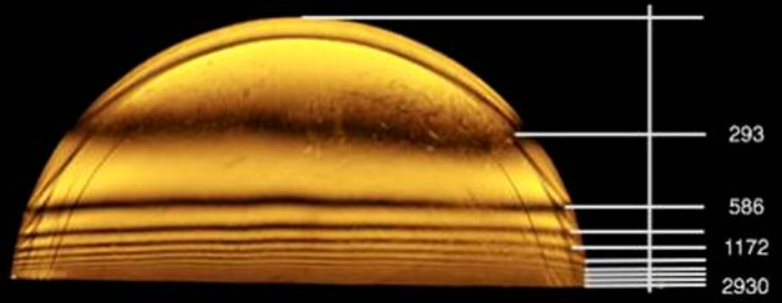
\includegraphics[width=0.8\linewidth]{bulle_monochromatique.png} 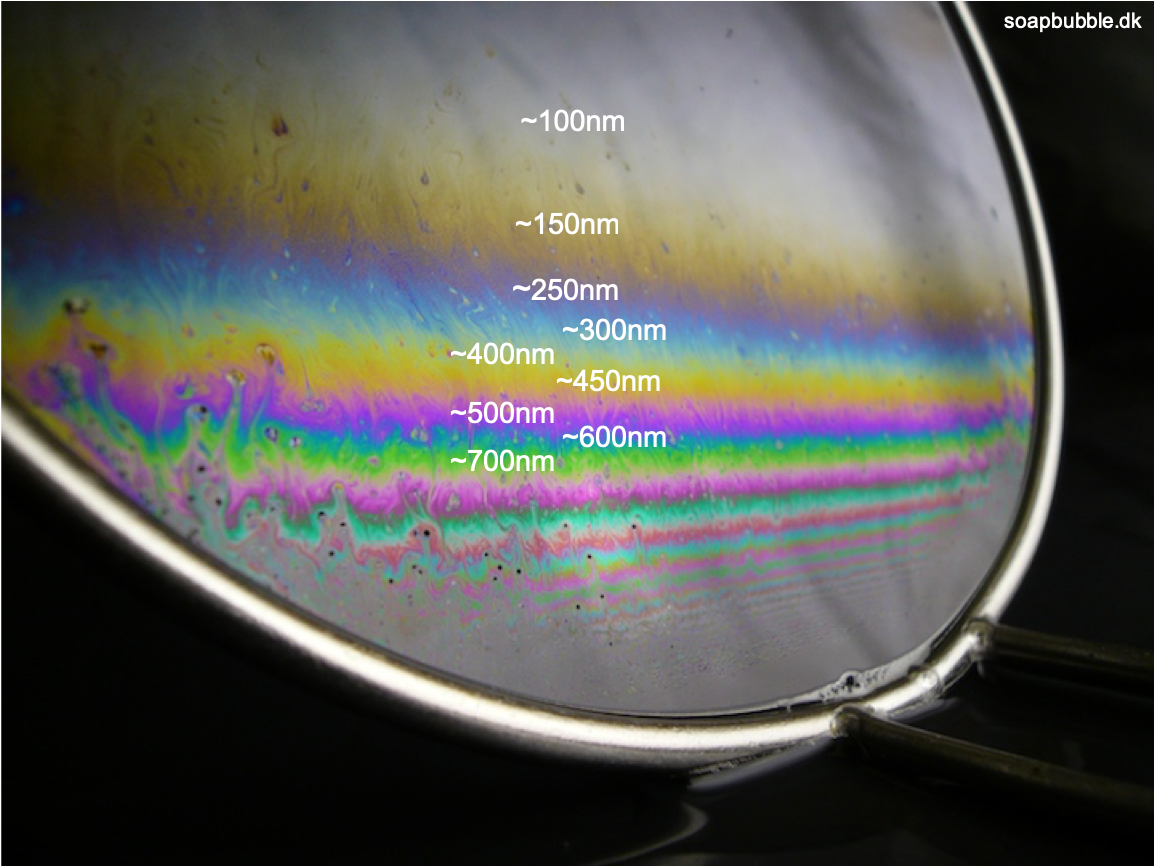
\includegraphics[width=0.8\linewidth]{bulle_savon_visible.png}

	\caption{En haut : demi-bulle de savon vue en lumière monochromatique. On observe des franges qui nous permettent d'estimer l'épaisseur du film en nm (à droite). En bas : photo d'un film de savon, cette fois-ci éclairé par une lumière blanche. Source : soapbubble.dk}
\end{figure}

\subsubsection{Lumière blanche : teintes de Newton}

Si l'on se place en lumière blanche, on observe une figure nettement plus complexe. Pourquoi ? Nous avons ici une source qui a une longueur de cohérence de l'ordre de la longueur d'onde, soit environ $\ell_c = 600$\,nm. On observe donc un brouillage des interférences pour les grandes épaisseurs. Les interférences sont toujours présentes mais elles sont brouillées, on parle de \textit{blanc d'ordre supérieur}.
\begin{remark}
	Pour les plus curieux.ses : le blanc d'ordre supérieur n'est pas analogue au blanc naturel : si l'on réalise son spectre, on pourra se rendre compte qu'il contient des pics à certaines longueurs d'onde, pour lesquelles les interférences sont constructives, et des creux, qui sont des longueurs d'onde pour lesquelles les interférences sont destructives.
\end{remark} 

\begin{figure}[htbp]
	\centering 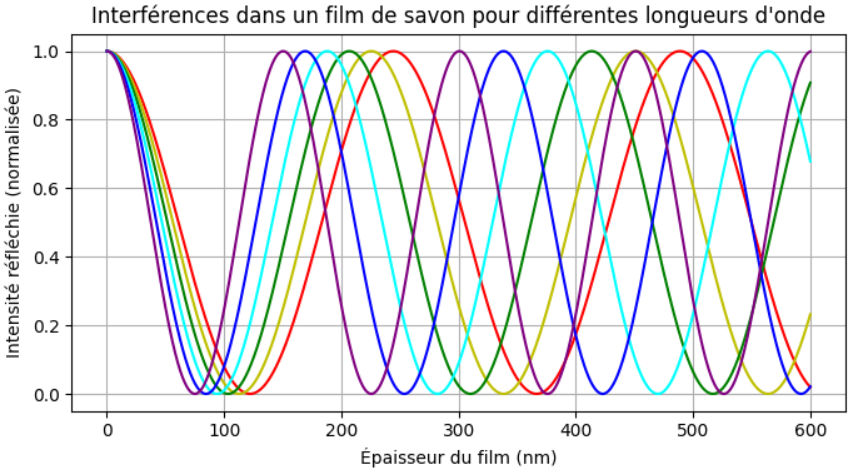
\includegraphics[width=0.8\linewidth]{couleurs_newton_1.png} 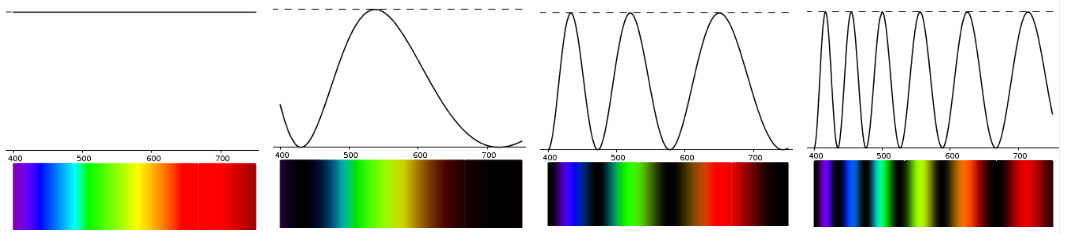
\includegraphics[width=\linewidth]{couleurs_newton_2.png}

	\caption{En haut : amplitude en fonction de l'épaisseur du film pour différentes longueurs d'onde. Plus l'épaisseur est élevée et plus les couleurs se mélangent, formant un blanc d'ordre supérieur. En bas : les spectres de chacune des couleurs des teintes de Newton.}
\end{figure}

Aux épaisseurs où l'on observe des interférences, on a ce que l'on appelle les teintes de Newton, qui correspondent à la superposition de couleurs de différentes longueurs d'onde comme indiqué sur la figure suivante. En effet on rappelle que les vibrations associées à deux longueurs d'ondes différentes sont incohérentes, donc elles n'interfèrent pas. On peut donc calculer les figures d'interférences pour chacune des longueurs d'onde, puis les superposer.

Ces couleurs apparaissent partout : vous y reconnaîtrez les couleurs d'un film d'essence sur une flaque, ou encore le bleu caractéristique des ailes du papillon Morpho vivant en Amazonie.

\begin{figure}[htbp]
	\centering 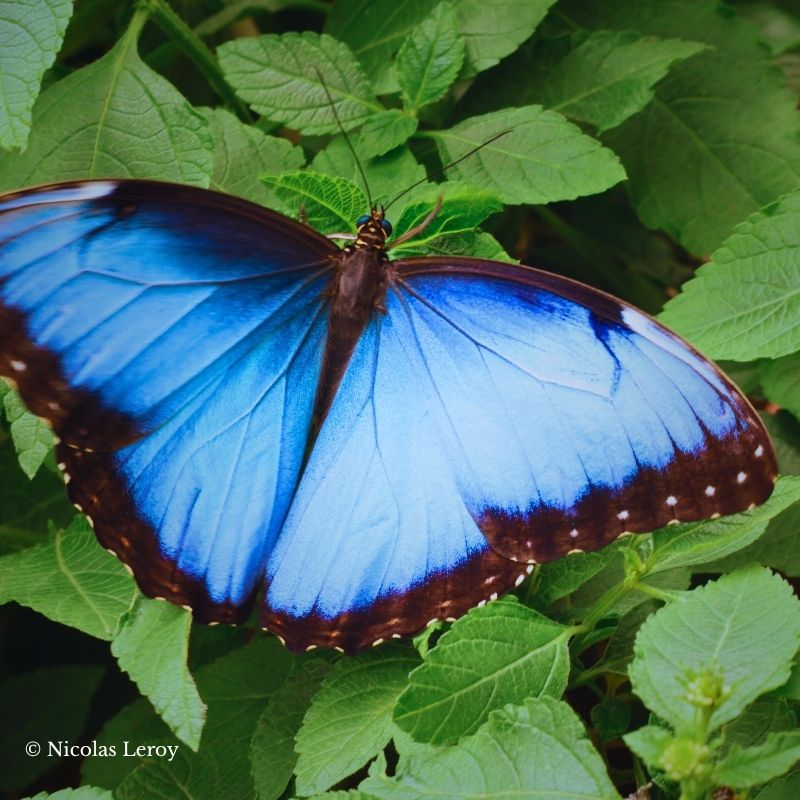
\includegraphics[width=0.5\linewidth]{papillon.jpg}
	\caption{Papillon Morpho. Source : Lepidoflora.}
\end{figure}

On peut dire que les teintes de Newton sont la signature du spectre lumineux émis par le Soleil. Si le spectre avait une forme différente, les couleurs que l'on verrait sur un film de savon seraient différentes. Ainsi, les interférences sont un outils formidable pour analyser les propriétés spectrales d'une source. Pour cela, on utilise un appareil permettant de contrôler précisément la différence de marche : un interféromètre.

\section{Interféromètre de Michelson}

\subsection{Présentation et principe de fonctionnement}

L'interféromètre de Michelson est un dispositif à deux miroirs, permettant de faire interférer deux rayons issus de la division d'un unique rayon lumineux initial. Le dispositif se présente comme suit :

\begin{figure}[htbp]
	\centering 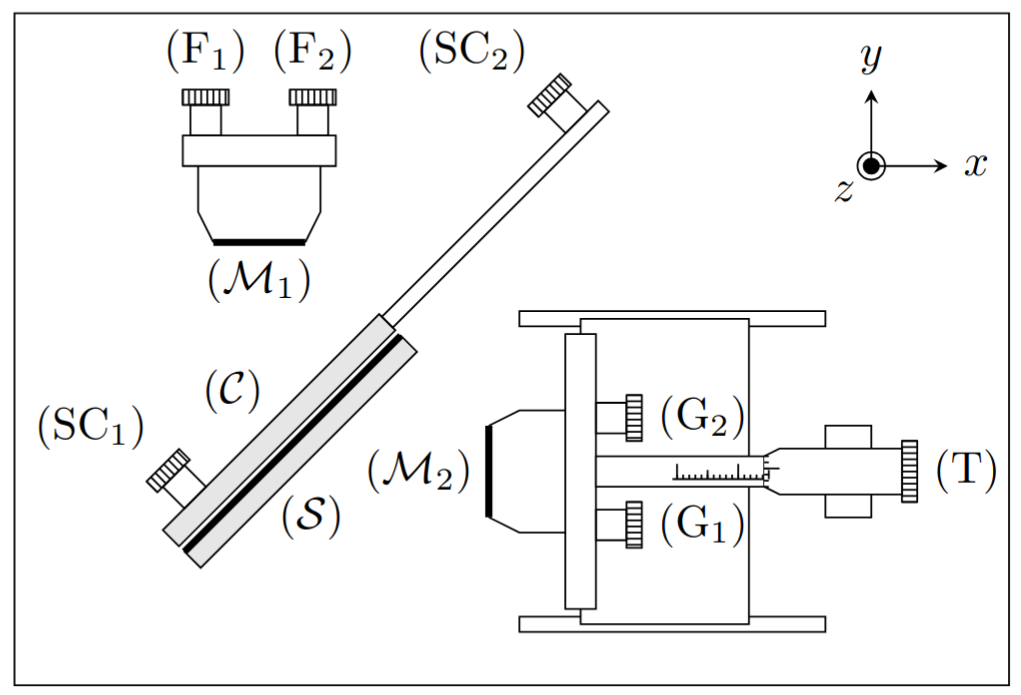
\includegraphics[width=0.5\linewidth]{schema_michelson.png} 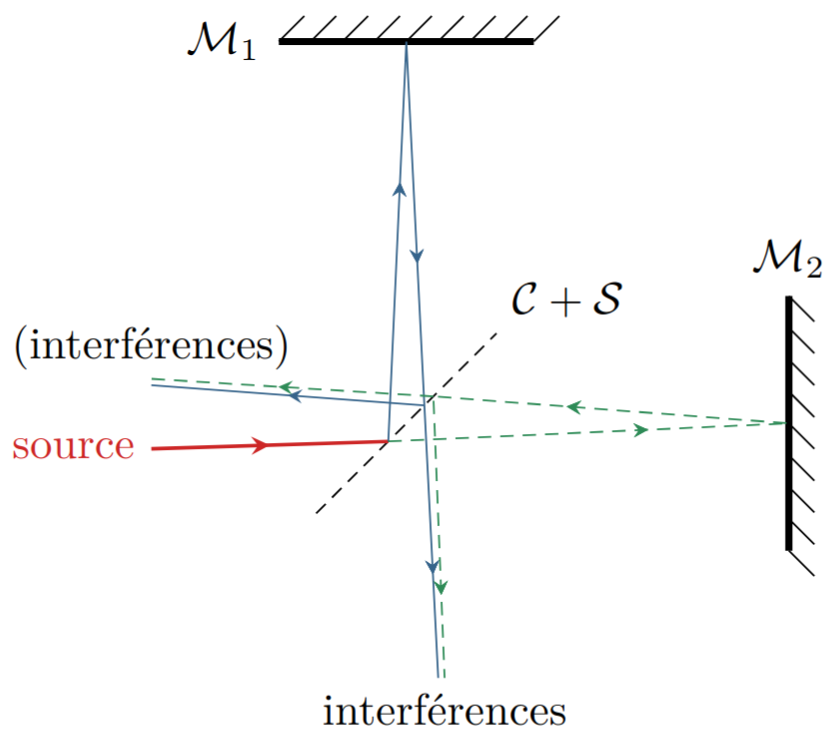
\includegraphics[width=0.45\linewidth]{michelson_principe.png}
 \caption{A gauche : schéma d'un interféromètre de Michelson. A droite : schéma de principe.}
\end{figure}

Deux miroirs $\mathcal{M}_1$ et $\mathcal{M}_2$ permettent de créer deux bras dans lesquels vont passer les deux rayons qui interfèrent. Pour créer ces deux rayons, on utilise une lame séparatrice $\mathcal{S}$. La lame compensatrice sert à compenser le chemin optique présent dans la séparatrice, et nous pourrons négliger son effet à ce niveau. L'ensemble se comporte comme une lame semi-réfléchissante : lorsqu'un rayon lumineux incident arrive sur la séparatrice, il subit une séparation en deux rayons d'intensité égale, le premier continuant son chemin sans être dévié, et le second étant réfléchi selon les lois de Snell-Descartes.

Afin de contrôler la différence de marche entre les rayons, on va modifier la longueur d'un rayon sur l'un des deux bras. Ceci est permis par le déplacement de l'un des deux miroirs, en l'occurence le miroir mobile $\mathcal{M}_2$, que l'on peut soit :
\begin{itemize}
	\item Déplacer horizontalement selon l'axe perpendiculaire au miroir par la vis (T) : on dit que l'on \textit{chariote}. On peut lire la position du miroir sur un vernier.
	\item Incliner le miroir à l'aide des vis (G$_1$) et (G$_2$).
\end{itemize}
Ces deux méthodes vont donner lieu à des figures d'interférences différentes. Nous nous intéresserons essentiellement à la première méthode dans ce cours, mais nous aborderons également la seconde méthode expérimentalement.

\subsection{Configuration en lame d'air ; anneaux d'égale inclinaison}

\begin{definition}
	On parle de configuration en \textit{lame d'air} lorsque les deux miroirs $\mathcal{M}_1$ et $\mathcal{M}_2$ sont orientés perpendiculairement, de sorte à ce que le symétrique $\mathcal{M}'_2$ de $\mathcal{M}_2$ par la séparatrice soit exactement parallèle à $\mathcal{M}_1$.
	On appelle alors épaisseur de la lame d'air la différence de longueur $e$ entre les deux bras.
\end{definition}

\paragraph{La méthode des images fictives}

Il est possible de ramener l'interféromètre à un dispositif linéaire en ne considérant plus la présence de la séparatrice, mais en représentant sur le schéma l'image de la source lumineuse $S$ et du miroir $\mathcal{M}_2$. Il s'agit d'un schéma équivalent qui permet de faciliter grandement les calculs.


\begin{figure}[htbp]
	\centering 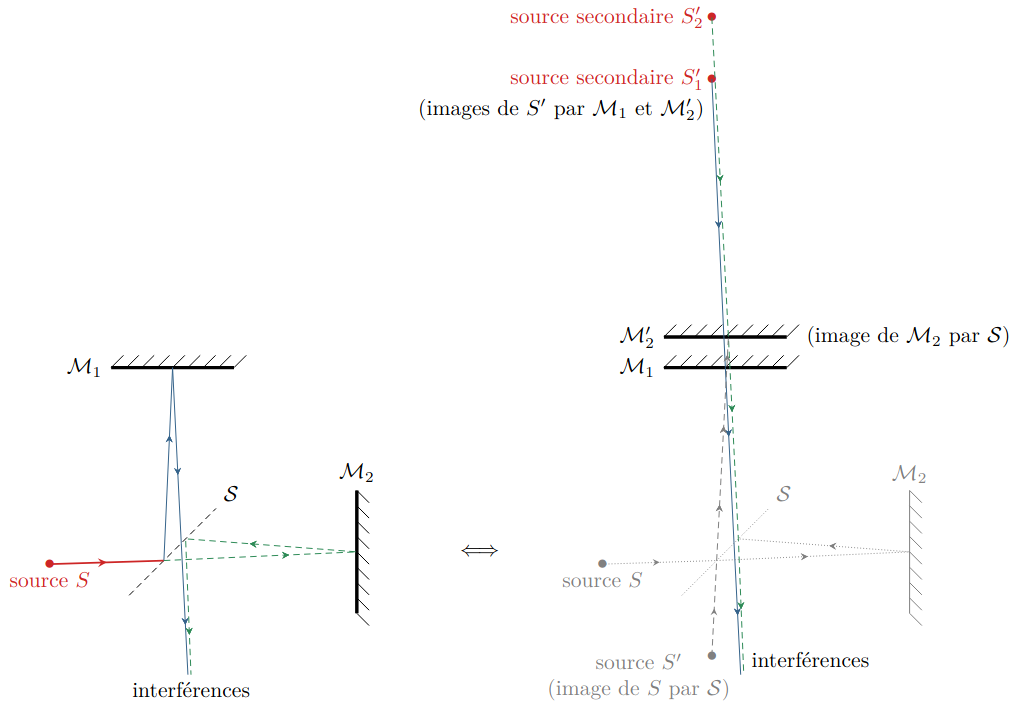
\includegraphics[width=\linewidth]{schema_equivalent_michelson.png}
	\caption{Schéma équivalent de l'interféromètre de Michelson en configuration de lame d'air. Source : poly de cours de Etienne Thibierge.}
\end{figure}

On constate alors que l'on se trouve dans la configuration vue en fin de chapitre dernier : des interférences entre deux sources ponctuelles cohérentes. L'écran se trouvant perpendiculairement à l'axe formé par les deux sources, on s'attend à observer des anneaux car la différence de marche est invariante par rotation autour de $S'_1 S'_2$.


\subsection{Conditions expérimentales d'observation}

Lorsque l'on met en oeuvre le dispositif expérimentalement, on éclaire d'abord l'interféromètre à l'aide d'un laser. On fait un premier constat :
\begin{proposition}
	Pour observer une figure d'interférences en lame d'air, il faut que les rayons atteignent les miroirs avec des inclinaisons variées. En pratique, on fait l'image de la source sur les miroirs à l'aide d'un condenseur.
\end{proposition}

Il convient donc d'élargir le faisceau laser et de le faire converger à l'aide d'une lentille, pour obtenir une variété d'inclinaisons sur les miroirs. On observe alors des anneaux en sortie de l'interféromètre, d'égale inclinaison $i_p$. Dans toute la suite, on note $i_p$ l'inclinaison de l'anneau d'ordre $p$.


On peut rajouter une lentille en sortie du dispositif : si l'on se place dans le plan focal image de la lentille, on voit que c'est là que les interférences sont les plus contrastées dans la cas où la source est étendue (lambe à vapeur de mercure, par exemple). On parle de localisation des interférences :
\begin{definition}
	Les interférences sont dites localisées lorsque l’utilisation d’une source étendue génère un contraste non uniforme dans le champ d’interférences.
	On appelle lieu de localisation la portion du champ d’interférences où le contraste est maximal.
\end{definition}

\begin{capex}
	Déterminer le lieu de localisation des interférences en lame d'air au vu des observations expérimentales.
\end{capex}

\subsection{Lame d'air en lumière monochromatique}

Nous allons maintenant nous intéresser plus précisément au cas de la lame d'air éclairée en lumière monochromatique (par exemple un laser). On constate que lorsque l'on se trouve au contact optique, il n'y a pas d'interférences : on observe un éclairage uniforme de l'écran : on parle de \textit{teinte plate}.

\begin{capex}
	Etablir l'expression de la différence de marche dans ce dispositif. En déduire la relation liant l'inclinaison des anneaux, l'épaisseur $e$ de la lame d'air, et l'ordre d'interférence $p$.
	L'ordre d'interférence le plus élevé se trouve-t-il au centre ou en périphérie de la figure d'interférences ?
\end{capex}

\begin{capex}
	Déterminer le rayon $r_p$ des anneaux, en fonction de $e,p$ et la focale $f'$ de la lentille de projection.
	Dans quel sens se déplacent les anneaux lorsqu'on chariote ?
\end{capex}

On conclut les propriétés suivantes :
\begin{proposition}
	Dans un interféromètre de Michelson en lame d’air, plus l’épaisseur de la lame d’air est grande, plus il y a d’anneaux visibles sur l’écran.
	Lorsque l’on s’éloigne du contact optique ($e$ augmente) : les anneaux se dilatent sur l’écran jusqu’à en sortir par le pourtour de la figure d’interférences alors que de nouveaux anneaux entrent par le centre ;
	Lorsque l’on se rapproche du contact optique ($e$ diminue) : les anneaux se contractent sur l’écran jusqu’à en sortir par le centre de la figure d’interférences alors que de nouveaux anneaux entrent par le pourtour.
\end{proposition}

\subsection{Spectroscopie interférentielle}

Bien que les propriétés des anneaux en lame d'air soient intéressantes, l'intérêt principal de l'interféromètre de Michelson en lame d'air réside dans son utilisation à l'aide de lumière non monochromatique : on peut alors utiliser les résultats expérimentaux pour obtenir des informations sur le spectre de la source lumineuse.








\subsection{Configuration en coin d'air : franges d'égale épaisseur}









\end{document}
